% =====================
% APPENDIX A: PROJECT BUDGET
% =====================
\chapter{PROJECT BUDGET}

The total budget required for the successful completion of the Uptime Tracker project is estimated to be between NPR 5,000 and NPR 10,000. Since this is a software-based project, the costs are primarily associated with cloud services, domain registration, and miscellaneous documentation expenses.

\section{Software and Development Tools}

All development tools used in this project are open-source and free:

\begin{table}[H]
    \centering
    \small
    \caption{Development Tools (No Cost)}
    \begin{tabular}{p{4cm}p{6cm}p{2.5cm}}
        \toprule
        \textbf{Tool} & \textbf{Description} & \textbf{Cost} \\
        \midrule
        Bun Runtime & JavaScript/TypeScript runtime & Free \\
        Next.js & React framework for frontend & Free \\
        Elysia.js & Backend web framework & Free \\
        PostgreSQL & Open-source database & Free \\
        Visual Studio Code & Code editor & Free \\
        Git & Version control system & Free \\
        Tailwind CSS & CSS framework & Free \\
        \midrule
        \multicolumn{2}{r}{\textbf{Subtotal}} & \textbf{Free} \\
        \bottomrule
    \end{tabular}
    \label{tab:dev_tools}
\end{table}

\section{Hosting and Cloud Services}

For deployment and hosting, the following services may be required:

\begin{table}[H]
    \centering
    \small
    \caption{Hosting and Cloud Services Cost}
    \begin{tabular}{p{4cm}p{5cm}p{3cm}}
        \toprule
        \textbf{Service} & \textbf{Description} & \textbf{Estimated Cost} \\
        \midrule
        Domain Registration & .com or .np domain (1 year) & NPR 1,500 - 2,500 \\
        VPS Hosting & Basic cloud server (3 months) & NPR 2,000 - 4,000 \\
        PostgreSQL Hosting & Managed database (optional) & Free tier available \\
        SSL Certificate & Let's Encrypt & Free \\
        \midrule
        \multicolumn{2}{r}{\textbf{Subtotal}} & \textbf{NPR 3,500 - 6,500} \\
        \bottomrule
    \end{tabular}
    \label{tab:hosting_services}
\end{table}

\textit{Note: Free-tier options from Vercel (frontend), Railway (backend), and Supabase (database) can reduce hosting costs to zero during development and initial deployment.}

\section{Total Budget Summary}

\begin{table}[H]
    \centering
    \small
    \caption{Total Estimated Budget}
    \begin{tabular}{p{6cm}p{4cm}}
        \toprule
        \textbf{Category} & \textbf{Estimated Cost} \\
        \midrule
        Development Tools & Free \\
        Hosting and Cloud Services & NPR 3,500 - 6,500 \\
        \midrule
        \textbf{Total Estimated Cost} & \textbf{NPR 3,500 - 6,500} \\
        \bottomrule
    \end{tabular}
    \label{tab:total_budget}
\end{table}

\textit{Note: The actual costs may vary depending on the hosting provider chosen and the duration of service usage. Using free-tier cloud services can significantly reduce the overall budget.}


% =====================
% APPENDIX B: PROJECT TIMELINE
% =====================
\chapter{PROJECT TIMELINE}

The project will be executed over a period of approximately 3 months, divided into several key phases. Each phase includes specific tasks and milestones to ensure steady progress toward project completion.




\section{Gantt Chart}

The Gantt chart in Figure \ref{fig:gantt_chart} provides a visual representation of the project timeline, showing task durations, dependencies, and key milestones.

\begin{figure}[H]
    \centering
    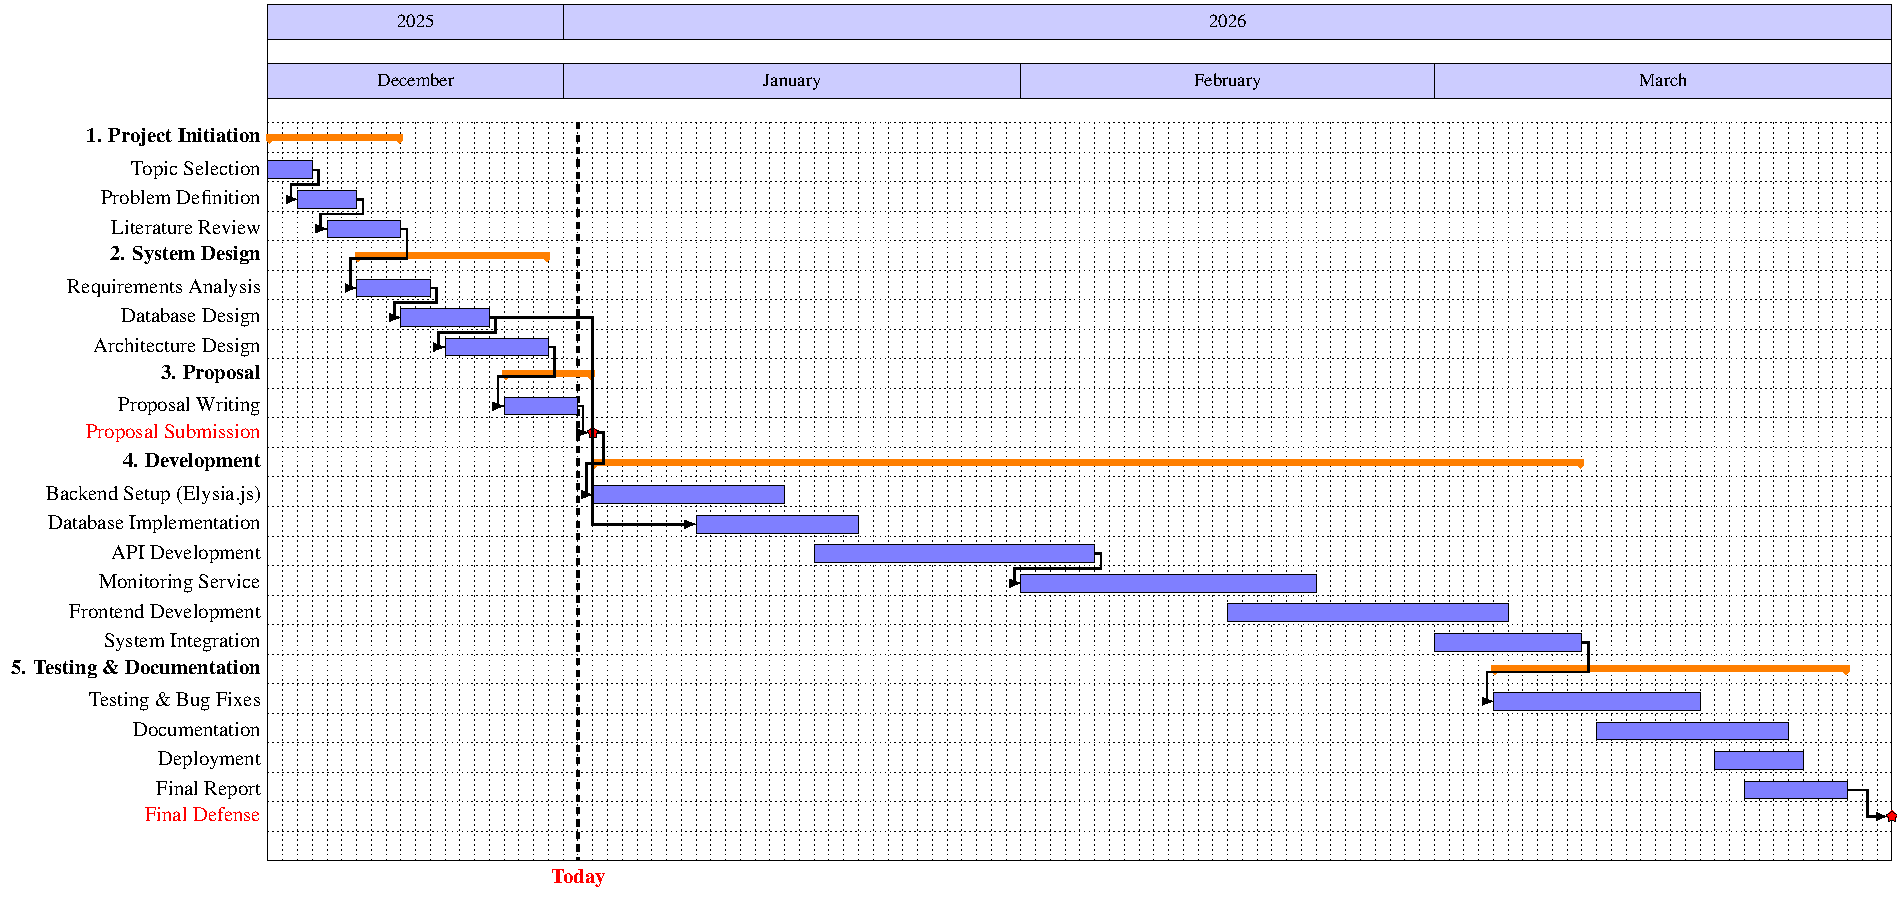
\includegraphics[width=\textwidth]{src/images/gantt/gantt.pdf}
    \caption{Project Gantt Chart}
    \label{fig:gantt_chart}
\end{figure}

\section{Milestone Summary}

Key project milestones are summarized in Table \ref{tab:milestones}:

\begin{table}[H]
    \centering
    \caption{Project Milestones}
    \begin{tabular}{llp{6cm}}
        \toprule
        \textbf{Milestone} & \textbf{Target Date} & \textbf{Deliverable} \\
        \midrule
        Project Start & December 12, 2025 & Topic selection and planning \\
        Design Complete & December 30, 2025 & Database schema and architecture \\
        Proposal Submission & January 2, 2026 & Complete project proposal \\
        Backend Complete & February 15, 2026 & Working API and monitoring service \\
        Development Complete & March 10, 2026 & Fully integrated application \\
        Final Report & March 28, 2026 & Complete project documentation \\
        Final Defense & March 31, 2026 & Project presentation and demo \\
        \bottomrule
    \end{tabular}
    \label{tab:milestones}
\end{table}

